% Kompilacja: lualatex main.tex  (albo xelatex)
\documentclass[aspectratio=169,professionalfonts,t]{beamer}

\usepackage{fontspec}
\usepackage[polish]{babel}
\usepackage{tikz}
\usepackage{amsmath}
\usepackage{booktabs}
\usepackage{tabularx}
\usepackage{array}
\usepackage{url}

\setsansfont{Calibri}[
  BoldFont = {Calibri Bold},
  ItalicFont = {Calibri Italic},
  BoldItalicFont = {Calibri Bold Italic}
]
\newfontfamily\calibriLight{Calibri Light}[
  ItalicFont = {Calibri Light Italic},
  BoldFont = Calibri,
  BoldItalicFont = {Calibri Italic}
]

% Kolory motywu Office z pliku PPTX.
\definecolor{poBlue}{HTML}{4472C4}

\setbeamercolor{normal text}{fg=black}
\setbeamercolor{frametitle}{fg=black}
\setbeamercolor{title}{fg=black}
\setbeamercolor{subtitle}{fg=black}
\setbeamercolor{item}{fg=black}
\setbeamercolor{subitem}{fg=black}
\setbeamercolor{subsubitem}{fg=black}
\setbeamercolor{structure}{fg=poBlue}

% Rozmiary PPTX przeskalowane do slajdu Beamera 160 mm x 90 mm.
\setbeamerfont{normal text}{family=\sffamily,size=\fontsize{13.2}{14.3}\selectfont}
\setbeamerfont{frametitle}{family=\calibriLight,size=\fontsize{20.8}{22.5}\selectfont}
\setbeamerfont{title}{family=\calibriLight,size=\fontsize{28.3}{30.6}\selectfont}
\setbeamerfont{subtitle}{family=\sffamily,size=\fontsize{11.3}{12.2}\selectfont}
\setbeamerfont{itemize/enumerate body}{parent=normal text}
\setbeamerfont{itemize/enumerate subbody}{parent=normal text}
\setbeamerfont{itemize/enumerate subsubbody}{parent=normal text}
\AtBeginDocument{\usebeamerfont{normal text}}

\makeatletter
\define@key{beamerframe}{t}[true]{%
  \beamer@frametopskip=0pt\relax
  \beamer@framebottomskip=0pt plus 1fill\relax
  \beamer@frametopskipautobreak=0pt\relax
  \beamer@framebottomskipautobreak=0pt plus 1fill\relax
}
\makeatother

\setbeamersize{text margin left=12.2mm, text margin right=12.2mm}
\setlength{\leftmargini}{3mm}
\setlength{\leftmarginii}{6mm}
\setlength{\leftmarginiii}{6mm}
\setlength{\itemsep}{2.4pt}
\setlength{\parsep}{0pt}
\setlength{\labelsep}{1.5mm}

% Beamer mierzy nagłówek przy \begin{document}, zanim zdefiniuje te polecenia.
\providecommand{\insertframetitle}{}
\providecommand{\insertframesubtitle}{}

\setbeamertemplate{navigation symbols}{}
\setbeamertemplate{frametitle}{}
\setbeamertemplate{itemize/enumerate body begin}{%
  \setlength{\topsep}{0pt}%
  \setlength{\partopsep}{0pt}%
}
\setbeamertemplate{itemize item}{\textbullet}
\setbeamertemplate{itemize subitem}{\textbullet}
\setbeamertemplate{itemize subsubitem}{\textbullet}

\setbeamertemplate{background canvas}{%
  
\includegraphics[width=\paperwidth,height=\paperheight]{tlo.png}%
}

% Pole tytułu z wzorca: x = 11 mm, y = 4,8 mm, wysokość 17,4 mm.
% Treść zaczyna się pod tym polem, na wysokości 24 mm.
\setbeamertemplate{headline}{%
  \begin{tikzpicture}[remember picture,overlay]
    \node[
      anchor=west,
      inner sep=0pt,
      outer sep=0pt,
      text width=135.6mm,
      align=left
    ] at ([xshift=12.2mm,yshift=-16.5mm]current page.north west) {%
      \usebeamerfont{frametitle}\usebeamercolor[fg]{frametitle}\insertframetitle
    };
  \end{tikzpicture}%
  \rule{0pt}{23.96mm}%
}

% Dolny margines zostawia miejsce na stopkę z tła; numer slajdu w prawym dolnym rogu.
\setbeamerfont{page number in head/foot}{size=\fontsize{7.5}{8.5}\selectfont}
\setbeamertemplate{footline}{%
  \begin{tikzpicture}[remember picture,overlay]
    \ifnum\insertframenumber>1\relax
      \node[
        anchor=south east,
        inner sep=0pt,
        outer sep=0pt
      ] at ([xshift=-5.0mm,yshift=5.0mm]current page.south east) {%
        \usebeamerfont{page number in head/foot}\insertframenumber
      };
    \fi
  \end{tikzpicture}%
  \rule{0pt}{8.93mm}%
}

% Slajd tytułowy: tytuł wyśrodkowany, dosunięty do dołu pola, podtytuł pod nim.
% \setbeamertemplate{title page}{%
%   \begin{tikzpicture}[remember picture,overlay]
%     \node[
%       anchor=south,
%       inner sep=0pt,
%       outer sep=0pt,
%       text width=117.6mm,
%       align=center
%     ] at ([yshift=-46.07mm]current page.north) {%
%       \usebeamerfont{title}\usebeamercolor[fg]{title}\inserttitle
%     };
%     \node[
%       anchor=north,
%       inner sep=0pt,
%       outer sep=0pt,
%       text width=117.6mm,
%       align=center
%     ] at ([yshift=-47.87mm]current page.north) {%
%       \usebeamerfont{subtitle}\usebeamercolor[fg]{subtitle}\insertsubtitle
%     };
%   \end{tikzpicture}%
% }

\newcommand{\smalltablefont}{\fontsize{9.4}{10.8}\selectfont}

\begin{document}

\title{Kalibracja prawdopodobieństw przez temperature scaling}
\subtitle{Etap 1 - prezentacja tematu}
\author{Paweł Gola}
\date{}

\begin{frame}
  \titlepage
\end{frame}

% --- 1. Opis problemu ---
\begin{frame}{Opis problemu}
  Współczesne sieci neuronowe często są źle skalibrowane: accuracy bywa wysoka, ale confidence odpowiedzi jest zawyżona.
  
  \vspace{0.5em}
  Publikacja pokazuje, że prostym środkiem naprawy może być skalowanie temperaturą.
  
  \vspace{1em}
  % \centering{C. Guo, G. Pleiss, Y. Sun, K. Q. Weinberger. \textit{On Calibration of Modern Neural Networks.} ICML 2017.}
  \centering{\textit{On Calibration of Modern Neural Networks}\\ Chuan Guo, Geoff Pleiss, Yu Sun, Kilian Q. Weinberger Proceedings of the 34th International Conference on Machine Learning, PMLR 70:1321-1330, 2017. }
\end{frame}

\begin{frame}{Podstawowe pojęcia}
  \begin{itemize}
    \item Logity
    \item Funkcja softmax
    \item Ujemny logarytm funkcji wiarygodności (ang. negative log-likelihood, NLL)
    \item Kalibracja
    \item Diagram niezawodności
    \item Oczekiwany błąd kalibracji (ang. expected calibration error, ECE)
  \end{itemize}
\end{frame}

% --- 2. Pojęcia (każde osobno) ---
\begin{frame}{Logity}
  Sieć klasyfikująca $K$ klas zwraca dla każdego obiektu wektor $K$ liczb rzeczywistych $\mathbf{z}=(z_1,\dots,z_K)$, zwanych logitami.
  
  Logity nie są prawdopodobieństwami, bo mogą być ujemne i nie sumują się do jedynki.
  
  Im większy logit, tym bardziej sieć skłania się ku danej klasie.

  \vspace{0.5em}
  Przewidywana klasa to indeks największego logitu: $\hat y=\arg\max_j z_j$.
\end{frame}

\begin{frame}{Funkcja softmax}
  Aby z logitów uzyskać prawdopodobieństwa, stosuje się znormalizowaną funkcję wykładniczą (softmax):
  \[
  p_j=\frac{\exp(z_j)}{\sum_{k=1}^{K}\exp(z_k)}.
  \]
  Wszystkie $p_j$ są dodatnie i sumują się do $1$.
  Wynik zależy wyłącznie od różnic między logitami: dodanie tej samej liczby do wszystkich logitów nie zmienia prawdopodobieństw.
\end{frame}

\begin{frame}{Ujemny logarytm funkcji wiarygodności (NLL)}
  NLL mierzy, jak dużą wagę model przypisał prawdziwej klasie:
  \[
  \mathrm{NLL}=-\sum_{i=1}^{n}\log p_{i,y_i}.
  \]
  Silnie karze pewne siebie pomyłki, dlatego jest naturalną funkcją celu przy dopasowaniu temperatury.
\end{frame}

\begin{frame}{Kalibracja}
  Model jest skalibrowany, gdy jego confidence odpowiada rzeczywistej częstości poprawnych odpowiedzi.
  Spośród stu predykcji z confidence $0{,}8$ powinno być poprawnych około osiemdziesięciu.
  \[
  \mathbb{P}\bigl(\hat Y=Y\mid\hat P=p\bigr)=p
  \quad\text{dla każdego }p\in[0,1].
  \]
  Accuracy i kalibracja to dwie różne własności: model może mieć wysoką accuracy i jednocześnie zawyżoną confidence.
\end{frame}

\begin{frame}{Diagram niezawodności}
  Przedział $(0,1]$ dzieli się na $M$ równych koszyków. W koszyku $B_m$:
  \[
  \mathrm{acc}(B_m)=\frac{1}{|B_m|}\sum_{i\in B_m}\mathbf{1}(\hat y_i=y_i),\qquad
  \mathrm{conf}(B_m)=\frac{1}{|B_m|}\sum_{i\in B_m}\hat p_i.
  \]
  \begin{columns}[c]
    \begin{column}{0.60\textwidth}
      Wykres accuracy względem confidence.
      Idealnie skalibrowany model leży na przekątnej; poniżej — nadmierne confidence, powyżej — niedostateczne.
    \end{column}
    \begin{column}{0.40\textwidth}
      \centering
      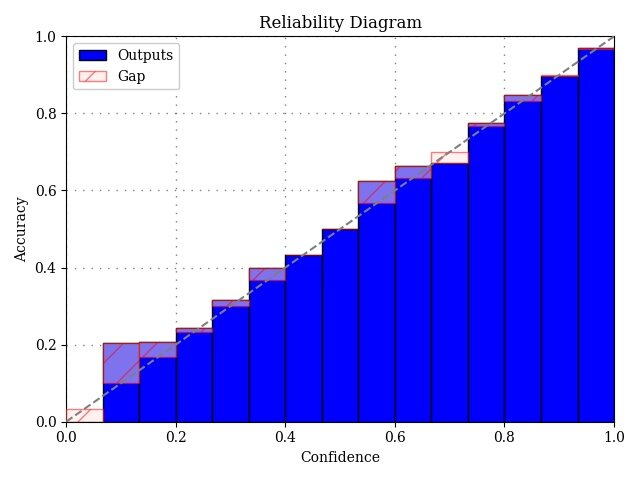
\includegraphics[height=0.40\textheight]{Reliability-diagrams.jpg}
    \end{column}
  \end{columns}
\end{frame}

\begin{frame}{Oczekiwany błąd kalibracji (ECE)}
  ECE jest średnią ważoną różnic między accuracy a confidence w koszykach:
  \[
  \mathrm{ECE}=\sum_{m=1}^{M}\frac{|B_m|}{n}\,\bigl|\mathrm{acc}(B_m)-\mathrm{conf}(B_m)\bigr|.
  \]
  ECE zależy od liczby koszyków i liczby obserwacji, dlatego należy je interpretować razem z NLL i diagramem niezawodności.
\end{frame}

% \begin{frame}{Accuracy}
%   Accuracy to odsetek obiektów sklasyfikowanych poprawnie.
%   Mówi, jak często sieć wskazuje właściwą klasę, ale nic nie mówi o tym, czy podawana confidence jest wiarygodna.
%   Przy skalowaniu temperaturą accuracy pozostaje niezmienione, bo dodatnia temperatura nie zmienia kolejności logitów.
% \end{frame}

% \begin{frame}{Confidence}
%   Confidence predykcji to największe z prawdopodobieństw po softmaxie: $\hat p=\max_j p_j$.
%   Wysoka confidence oznacza, że model silnie faworyzuje jedną klasę względem pozostałych.
%   Problem badany w projekcie dotyczy właśnie tego, czy ta wartość odpowiada rzeczywistej częstości poprawnych odpowiedzi.
% \end{frame}

% --- 3. Temperature scaling ---

\begin{frame}{}
  \begin{tikzpicture}[remember picture,overlay]
    \node[anchor=center] at (current page.center) {%
      \usebeamerfont{title}\usebeamercolor[fg]{title}Temperature scaling%
    };
  \end{tikzpicture}
\end{frame}

\begin{frame}{Temperature scaling}
  Wszystkie logity dzielimy przez jedną dodatnią temperaturę $T$ przed softmaxem:
  \[
  p_j(T)=\frac{\exp(z_j/T)}{\sum_{k=1}^{K}\exp(z_k/T)},\qquad T>0.
  \]
  \begin{itemize}
    \item $z_j$ — logit klasy $j$; $K$ — liczba klas; $T$ — jedyny dopasowywany parametr.
    \item Dla $T=1$ odzyskujemy pierwotne prawdopodobieństwa.
    \item Dla $T>1$ rozkład się spłaszcza i confidence maleje; dla $T<1$ confidence rośnie.
  \end{itemize}
  % Parametry sieci pozostają niezmienione: temperaturę dopasowujemy dopiero po treningu przez minimalizację NLL na zbiorze kalibracyjnym.
\end{frame}

% --- 4. Przykład obliczeniowy ---
\begin{frame}{Przykład obliczeniowy}
  Weźmy dwie klasy z logitami $z_1=2$ i $z_2=0$.
  \begin{itemize}
    \item Przy $T=1$: $p_1\approx0{,}881$, $p_2\approx0{,}119$, więc confidence wynosi $0{,}881$.
    \item Przy $T=2$: $p_1\approx0{,}731$, $p_2\approx0{,}269$, więc confidence spada do $0{,}731$.
  \end{itemize}
  Dzielenie przez $T>0$ zachowuje kolejność logitów, więc $\arg\max$ się nie zmienia.
  Skalowanie temperaturą nie zmienia ani jednej predykcji: zmieniają się tylko confidence, NLL i ECE.
\end{frame}

\begin{frame}{Dopasowanie temperatury}
  Temperaturę wybiera się przez minimalizację NLL na zbiorze kalibracyjnym:
  \[
  T^\ast=\arg\min_{T>0}\;\sum_{i=1}^{n}\Bigl[\log\sum_{k}\exp\!\bigl(z_{ik}/T\bigr)-z_{i,y_i}/T\Bigr].
  \]
  Po zastąpieniu $T$ przez $\beta=1/T$ funkcja celu jest wypukła, więc minimum jest jedno.
\end{frame}



% --- 5. Odtwarzany fragment ---
\begin{frame}{Odtwarzany fragment}
  Odtwarzany będzie wynik z tabeli 1 publikacji dla sieci LeNet-5 na CIFAR-10: ECE wynosi $3{,}02\%$ przed kalibracją i $0{,}93\%$ po skalowaniu temperaturą.
  
  CIFAR-10 to kolorowe obrazy $32\times32$ z dziesięcioma klasami: $50\,000$ obrazów treningowych i $10\,000$ testowych.
  
  Zastosowany podział zgodny z publikacją: trening $45\,000$, walidacja $5\,000$, test $10\,000$.
  
  Temperatura dostosowywana na walidacji, a accuracy, NLL i ECE oceniana na teście.
\end{frame}

% \begin{frame}{Odtwarzany fragment: sieć i trening}
%   Publikacja nie podaje szczegółów treningu LeNet-5, więc wartości ustalamy z góry przed oceną na teście.
%   \begin{itemize}
%     \item Architektura: dwie warstwy splotowe, warstwy łączące przez maksimum oraz warstwy w pełni połączone $400\to120\to84\to10$.
%     \item Optymalizator: SGD z pędem $0{,}9$; szybkość uczenia $0{,}01$; porcje po $128$.
%     \item Co najwyżej $60$ epok; wybieramy epokę o najmniejszym błędzie walidacyjnym.
%   \end{itemize}
%   Wykonujemy pięć treningów z różnymi ziarnami i podajemy średnią oraz rozrzut wyników.
% \end{frame}

\begin{frame}{Zmiany względem publikacji}
  \begin{itemize}
    \item Implementacja w PyTorch; publikacja używała biblioteki Torch7.
    \item Parametry treningu i wariant LeNet-5; publikacja nie podaje szczegółów treningu LeNet-5
    \item Odtwarzanie tylko stanu przed skalowaniem i po nim; pominięcie pozostałych metod kalibracji.
  \end{itemize}
\end{frame}

\begin{frame}{Spodziewane różnice w wynikach}
  Brak pełnego opisu treningu może spowodować inny ECE przed kalibracją niż $3{,}02\%$.
  Porównanie z publikacją prowadzone będzie jakościowowedług następujących kryteriów:
  \begin{itemize}
    \item accuracy nie zmienia się po skalowaniu,
    \item ECE i NLL na teście maleją,
    \item temperatura jest większa od $1$, jeśli sieć ma nadmiernie wysokie confidence,
    \item diagram niezawodności po kalibracji leży bliżej przekątnej.
  \end{itemize}
\end{frame}

% --- 6. Badanie ---
\begin{frame}{Badanie: pytanie i hipotezy}
  \textbf{Pytanie:} czy jedna temperatura poprawia kalibrację małej sieci i jak liczba przykładów kalibracyjnych wpływa na wiarygodność tej poprawy?
  \vspace{0.5em}
  \begin{itemize}
    \item \textbf{H1.} Temperatura dopasowana na zbiorze kalibracyjnym zmniejsza NLL na teście, a ECE maleje, jeśli sieć była źle skalibrowana. Accuracy nie zmienia się.
    \item \textbf{H2.} Przy $30$ obiektach temperatura jest mocno zmienna. Przy $100$ i $300$ obiektach zmienność maleje, a poprawa NLL jest częstsza i bardziej przewidywalna.
  \end{itemize}
\end{frame}

\begin{frame}{Badanie: dane i podział}
  Zbiór \emph{digits} z biblioteki scikit-learn: $1797$ obrazów cyfr $8\times8$ (64 cechy) z dziesięcioma klasami.
  
  \vspace{0.5em}
  Dane dzielone są warstwowo na trzy rozłączne części z ustalonym ziarnem:
  \begin{itemize}
    \item trening sieci: $900$ obiektów,
    \item zbiór kalibracyjny: $300$ obiektów (pula próbek $30$, $100$ i $300$),
    \item test końcowy: $597$ obiektów.
  \end{itemize}
\end{frame}

\begin{frame}{Badanie: sieć, metody i miary}
  Mała sieć MLP: $64$ wejścia, jedna warstwa ukryta z $64$ neuronami ReLU oraz $10$ wyjść.
  Uczenie entropią krzyżową optymalizatorem Adam przez $150$ epok; pięć treningów z różnymi ziarnami.
  \begin{itemize}
    \item Metody: punkt odniesienia ($T=1$) oraz model po skalowaniu temperaturą ($T^\ast$).
    \item Miary: accuracy, średnia NLL, ECE z $M=15$ oraz diagram niezawodności.
  \end{itemize}
\end{frame}

\begin{frame}{Badanie: część A i część B}
  \textbf{Część A.} Temperatura dopasowana na całej puli $300$ obiektów i porównanie modelu przed skalowaniem oraz po nim na teście.
  Ta część sprawdza, czy jedna temperatura poprawia kalibrację małej sieci.

  \vspace{0.5em}
  \textbf{Część B.} Dla wielu zagnieżdżonych próbek $30$, $100$ i $300$ obiektów dopasowanie $T$ i ocenianie wyników na tym samym teście.
  Zaprezentowanie rozrzutu temperatur oraz odsetek losowań, w których skalowanie poprawiło NLL i ECE.
\end{frame}

% --- 7. Kontrola, granice, wykonalność ---
\begin{frame}{Kontrola przecieku i granice wnioskowania}
  Temperatura, liczba epok i liczba koszyków ECE ustalana przed oceną na teście; test służy wyłącznie do końcowej oceny.
  Zbiór kalibracyjny nie bierze udziału w treningu sieci, a normalizacja jest obliczana tylko na treningu.
  \begin{itemize}
    \item Wnioski dotyczą jednej małej architektury i jednego zbioru, więc nie są uogólniane na głębokie sieci.
    \item Mały zbiór testowy czyni ocenę ECE niepewną, zwłaszcza przy niewielkiej liczbie pomyłek.
    \item Próbki $30$ i $100$ pochodzą z tej samej puli $300$ obiektów, więc nie są niezależne.
  \end{itemize}
\end{frame}

\begin{frame}{Wykonalność}
  CIFAR-10 z torchvision, \emph{digits} z scikit-learn.
  
  \vspace{0.5em}
  Biblioteki: PyTorch, Probmetrics, NumPy, scikit-learn i Matplotlib.
  
  \vspace{0.5em}
  Zakres odtwarzania i badania ograniczony jest do małej architektury i małego zbioru, aby było możliwe uruchomienie w Google Colab lub na laptopie.
\end{frame}

\begin{frame}{Próba uruchomienia}
  LeNet-5 na CIFAR-10, $200$ epok (checkpoint: epoka $184$), $T^\ast=1{,}1309$.
  \vspace{0.4em}
  \begin{columns}[c]
    \begin{column}{0.30\textwidth}
      \centering
      \smalltablefont
      \begin{tabular}{@{}lcc@{}}
        \toprule
        & Przed ($T=1$) & Po skalowaniu \\
    \midrule
    Accuracy & $74{,}06\%$ & $74{,}06\%$ \\
    NLL & $0{,}7561$ & $0{,}7486$ \\
    ECE & $2{,}91\%$ & $1{,}02\%$ \\
        \bottomrule
      \end{tabular}
    \end{column}
    \begin{column}{0.34\textwidth}
      \raggedleft
      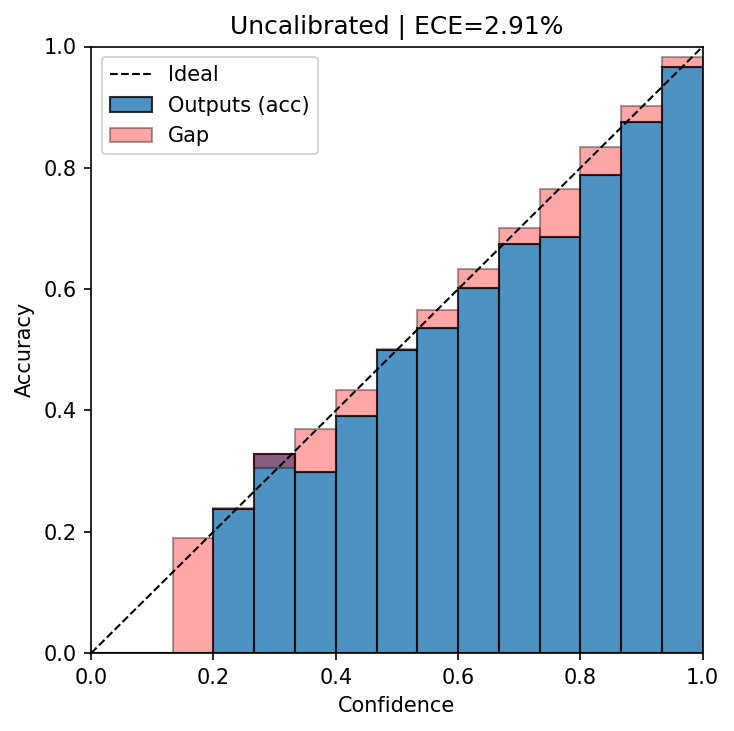
\includegraphics[height=0.48\textheight]{reliability_uncalibrated.png}
    \end{column}
    \begin{column}{0.30\textwidth}
      \centering
      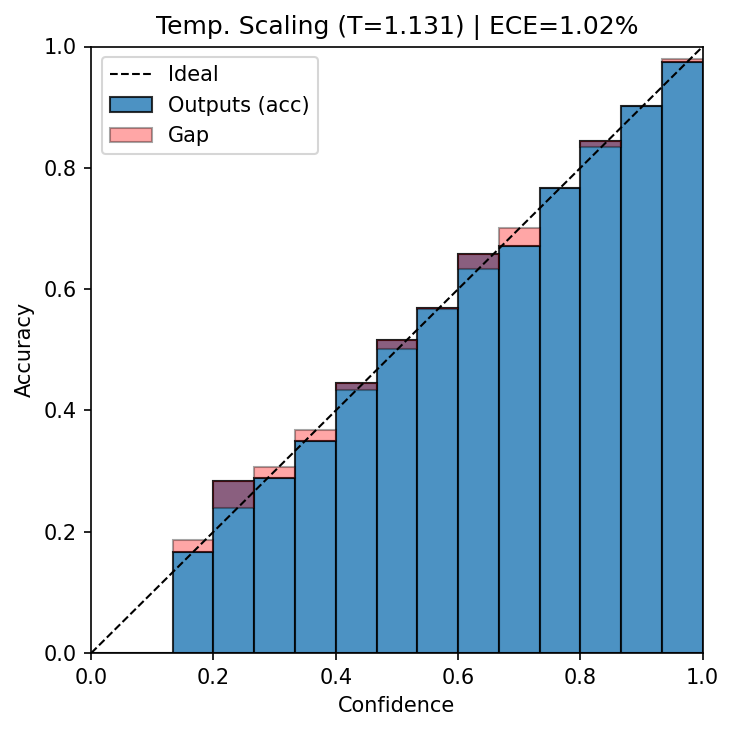
\includegraphics[height=0.48\textheight]{reliability_temperature_scaling.png}
    \end{column}
  \end{columns}
\end{frame}

\begin{frame}{Źródła}
  \begin{itemize}
    \item Chuan Guo, Geoff Pleiss, Yu Sun, Kilian Q. Weinberger. \textit{On Calibration of Modern Neural Networks.} ICML 2017.
    \item CIFAR-10 dataset: \url{https://www.cs.toronto.edu/~kriz/cifar.html}
    \item digits dataset: \url{https://scikit-learn.org/stable/modules/generated/sklearn.datasets.load_digits.html}
    \item Implementacja temperature scaling: \url{https://github.com/probkit/probmetrics}
  \end{itemize}
\end{frame}

\begin{frame}{}
  \begin{tikzpicture}[remember picture,overlay]
    \node[anchor=center] at (current page.center) {%
      \usebeamerfont{title}\usebeamercolor[fg]{title}Dziękuję za uwagę%
    };
  \end{tikzpicture}
\end{frame}

\end{document}
